\chapter{Tecnologias e Ferramentas Utilizadas}
\label{ch::tecno-ferr}

\section{Introdução}
\label{sec::tecno-ferr:intro}

O projeto apresentado só foi possível ser concluído devido à existência de tecnologias e ferramentas, assim como de materiais, os quais se revelaram essenciais.

Em particular, este Capítulo aborda:

\begin{itemize}
    \item O \textit{software} de reconstrução de hologramas;
    \item A escolha da linguagem de programação para o projeto;
    \item O \ac{SDK} de codificação de imagens no formato JPEG2000;
    \item O \textit{hardware} utilizado;
    \item Os hologramas testados.
\end{itemize}


\section{Tecnologias e Ferramentas}
\label{sec::tecno-ferr:tecno-ferr}

O desenvolvimento do projeto envolveu o trabalho conjunto de diversas ferramentas, nomeadamente Python 3, \textit{Kakadu Software} e \textit{software} escrito no âmbito do projeto JPEG Pleno.

\subsection{Software de Reconstrução de Hologramas e sua Transcrição para Python}

Do 80\textordmasculine~Encontro do Grupo JPEG, realizado em Berlim entre 7 e 13 de julho de 2018, resultou um software desenvolvido por Antonin Gilles e Patrick Gioia, do \textit{Institute of Research \& Technology b<>com}. O respetivo código, fornecido pela professora orientadora, encontra-se implementado em MATLAB.

Dada a ausência de uma licença do MATLAB para utilizar este \textit{sofware} desenvolvido no âmbito do JPEG Pleno, foi necessário transcrever o código para uma nova linguagem de programação. Neste sentido, optou-se pelo Python 3.

% Sendo uma linguagem , de utilização gratuita e com a vantagem de ser mais eficiente face ao MATLAB, 

O recurso a Python apresenta uma miríade de vantagens, entre elas:
\begin{itemize}
    \item Linguagem \textit{open source};
    \item Utilização e distribuição gratuita da linguagem;
    \item Maior eficiência face ao MATLAB;
    \item Utilização comum no contexto de processamento multimédia e respetivos projetos;
    \item Vasto leque de bibliotecas, facilitando a implementação de \textit{software} específico;
    \item Abundância de documentação;
    \item Forte comunidade \textit{online} de suporte.
\end{itemize}

A escolha do Python foi, portanto, natural no âmbito do presente projeto.

Durante a fase de transcrição decorreu uma atualização do Python, tendo sido a última versão do código executada e testada na versão 3.8.2 em três distribuições GNU/Linux de 64 bits: Ubuntu 18.04 LTS, Fedora 31 e Linux Mint 20.

\subsection{\textit{Kakadu Software}}
\label{ssec::tecno-ferr:tecno-ferr:kdu}
Uma vez que o JPEG2000 é o formato alvo deste projeto, e tendo em conta a dificuldade encontrada em projetos anteriores no contexto da holografia em utilizar a ferramenta \textit{FFmpeg}, foi recomendado pela professora orientadora a utilização do \textit{Kakadu Software}.

Este é um \ac{SDK} para codificação e descodificação de imagens com recurso ao formato JPEG2000, segundo o \textit{standard} pela \ac{JPEG}.

Os comandos deste \ac{SDK} de relevo para o projeto são os seguintes:

\begin{enumerate}
    \item \texttt{kdu\_compress}: codifica uma imagem para o formato JPEG2000.\\
    Sintaxe:
    \begin{minted}[breaklines,frame=lines]{bash}
kdu_compress -i input_file -o output_file -rate n Cycc=<yes|no> -precise -quiet
    \end{minted}
    onde:
    \begin{itemize}
        \item \verb|-i input_file|: imagem de \textit{input};
        \item \verb|-o output_file|: ficheiro de \textit{output};
        \item \verb|-rate n|: número de \textit{bits} por amostra ($n$ pode ser um número flutuante);
        \item \verb#Cycc=<yes|no>#: \verb|yes| caso seja usada a codificação com transformada de cor de \ac{RGB} para YCbCr, \verb|no| em caso contrário;
        \item \verb|-precise|: força o uso de representações de 32 \textit{bits};
        \item \verb|-quiet|: suprime o \textit{output} do programa.
    \end{itemize}
    
    \item \texttt{kdu\_expand}: descodifica uma imagem no formato JPEG2000.\\
    Sintaxe:
    \begin{minted}[breaklines,frame=lines]{bash}
kdu_expand -i input_file -o output_file -rate n -quiet
    \end{minted}
    onde:
    \begin{itemize}
        \item \verb|-i input_file|: imagem de \textit{input};
        \item \verb|-o output_file|: ficheiro de \textit{output};
        \item \verb|-rate n|: número de \textit{bits} por amostra ($n$ pode ser um número flutuante);
        \item \verb|-quiet|: suprime o \textit{output} do programa.
    \end{itemize}
\end{enumerate}

% 'kdu_compress -i {} -o {} -rate {} Cycc={} -precise -quiet'
% 'kdu_expand -i {} -o {} -rate {} -precise -quiet'

\section{Materiais Utilizados}
\label{sec::tecno-ferr:materiais}

\subsection{\textit{Hardware}}
\label{ssec::tecno-ferr:materiais:hardware}

De notar que esta implementação do \textit{software} de reconstrução de hologramas requer computadores com especificações mais generosas.

Para este projeto, dois computadores em particular executaram as várias iterações de desenvolvimento do \textit{software} transcrito em Python:
\begin{enumerate}
    \item \textit{Desktop}: processador Ryzen\texttrademark~7 2700X \@ 3.7--4.3GHz, placa gráfica NVidia\textsuperscript{\textregistered} Quadro K5000 (4GB), memória RAM de 32GB e \textit{swap} de 96GB, armazenamento SSD de 1TB;
    \item Portátil: Intel\textsuperscript{\textregistered}~Core\texttrademark~i5-10210U \@ 1.6--4.2GHz, memória RAM de 16GB e \textit{swap} de 8GB, armazenamento SSD de 512GB.
\end{enumerate}

\subsection{Hologramas}
\label{ssec::tecno-ferr:materiais:hologramas}

Os hologramas reconstruidos com o \textit{software} desenvolvido no âmbito deste projeto são fornecidos pelo \textit{Institute of Research \& Technology b<>com}. De entre os disponíveis, foram utilizados os seguintes hologramas com respetivas características resumidas na Tabela \ref{tab:holo-specs}:

\begin{enumerate}
    \item \texttt{Dices4k} (Figura \ref{fig:bcom_dices4k});
    \item \texttt{DiffuseCar4k} (Figura \ref{fig:bcom_diffuseCar4k});
    \item \texttt{Piano4k} (Figura \ref{fig:bcom_piano4k}).
\end{enumerate}


\begin{table}[!htbp]
    \centering
    \caption{Especificações dos hologramas.}
    \label{tab:holo-specs}
    \begin{tabular}{r c c c c c c}
        \toprule
        Holograma & \verb|size| & \verb|pitch| & \verb|r| & \verb|g| & \verb|b| & \verb|z| \\
        \midrule
        \texttt{Dices4k} & 4096$\times$4096 & \SI{0.4}{} & \SI{640}{} & \SI{532}{} & \SI{473}{} & \SI{0.164}{} -- \SI{0.328}{} \\
        %\hline
        \texttt{DiffuseCar4k} & 4096$\times$4096 & \SI{0.4}{} & \SI{640}{} & \SI{532}{} & \SI{473}{} & \SI{0.110}{} -- \SI{0.250}{} \\
        %\hline
        \texttt{Piano4k} & 4096$\times$4096 & \SI{0.4}{} & \SI{640}{} & \SI{532}{} & \SI{473}{} & \SI{0.170}{} -- \SI{0.313}{} \\
        \bottomrule
    \end{tabular}
    %\bigskip
    \subcaption*{}
    \begin{tabular}{>{\ttfamily}r @{~:~~} l l}
        size & Resolução & (em pixeis) \\
        pitch & \textit{Pixel pitch} & (em \SI{}{\micro\meter}) \\
        r & Comprimento de onda vermelho & (em \SI{}{\nano\meter}) \\
        g & Comprimento de onda verde & (em \SI{}{\nano\meter}) \\
        b & Comprimento de onda azul & (em \SI{}{\nano\meter}) \\
        z & Intervalo de localização da cena & (em \SI{}{\centi\meter}) \\
    \end{tabular}
\end{table}



\begin{figure}
    \centering
    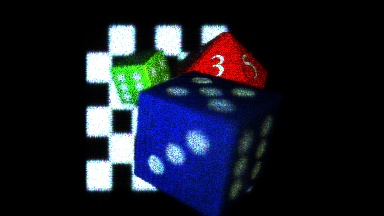
\includegraphics[width=\textwidth]{bcom_dices4k.jpg}
    \caption{Holograma \texttt{Dices4k} (imagem original).}
    \label{fig:bcom_dices4k}
\end{figure}

\begin{figure}
    \centering
    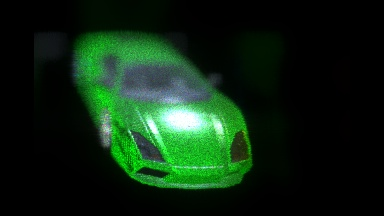
\includegraphics[width=\textwidth]{bcom_diffuseCar4k.jpg}
    \caption{Holograma \texttt{DiffuseCar4k} (imagem original).}
    \label{fig:bcom_diffuseCar4k}
\end{figure}

\begin{figure}
    \centering
    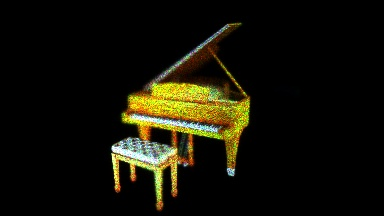
\includegraphics[width=\textwidth]{bcom_piano4k.jpg}
    \caption{Holograma \texttt{Piano4k} (imagem original).}
    \label{fig:bcom_piano4k}
\end{figure}


\section{Conclusões}
\label{sec::tecno-ferr:conclusao}

Após a seleção das tecnologias e materiais, conforme supra-mencionados, ir-se-á proceder no Capítulo \ref{ch::imp-test} ao delineamento da estratégia de investigação do projeto, a qual está intimamente ligada às escolhas apresentadas no presente Capítulo, entre elas a escolha da linguagem Python para transcrição do \textit{software} original de reconstrução de hologramas, o \ac{SDK} para realizar a codificação no formato JPEG2000 e os hologramas testados.
